\documentclass[simplex.tex]{subfiles}
% DO NOT INCLUDE PREAMBLES/PACKAGES HERE!!
% packages are inherited from preamble.tex; you can compile this on its own
\begin{document}
\subsection{FlashX}

%%%%%% April
This month, we improve FlashR deployment to simplify the use of FlashR in
a production environment. First, we integrate FlashR into Jupyter Notebook.
As such, users can analyze large datasets stored on a server, simply using
a Web browser. Figure \ref{fig:FlashX2} shows an example of using this
environment to compute singular value decomposition on a graph with billions
of vertices and generate the screeplot for singular values. In addition,
we deploy FlashR in docker to enable FlashR to run in various environments
easily, such as Macbook, Windows laptops and clouds.

\begin{figure}[!h]
\begin{cframed}
\centering
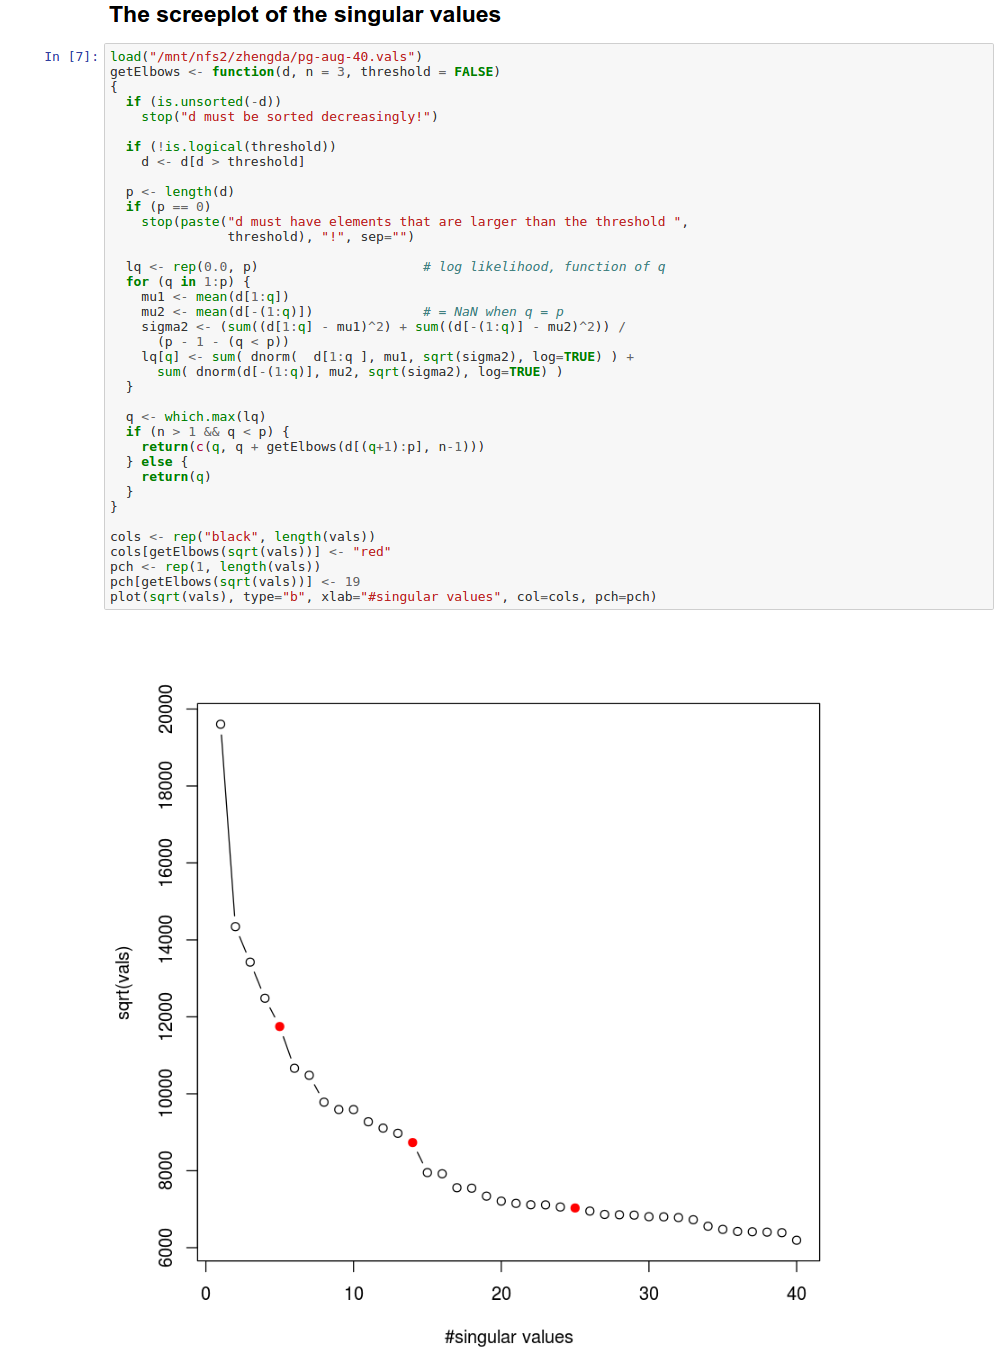
\includegraphics[width=0.6\textwidth]{../../figs/PG-screeplot.png}
\caption{Generate a screeplot for singular values of a graph with billions
	of vertices.}
\label{fig:FlashX2}
\end{cframed}
\end{figure}

\end{document}
